\documentclass[1p]{elsarticle_modified}
%\bibliographystyle{elsarticle-num}

%\usepackage[colorlinks]{hyperref}
%\usepackage{abbrmath_seonhwa} %\Abb, \Ascr, \Acal ,\Abf, \Afrak
\usepackage{amsfonts}
\usepackage{amssymb}
\usepackage{amsmath}
\usepackage{amsthm}
\usepackage{scalefnt}
\usepackage{amsbsy}
\usepackage{kotex}
\usepackage{caption}
\usepackage{subfig}
\usepackage{color}
\usepackage{graphicx}
\usepackage{xcolor} %% white, black, red, green, blue, cyan, magenta, yellow
\usepackage{float}
\usepackage{setspace}
\usepackage{hyperref}

\usepackage{tikz}
\usetikzlibrary{arrows}

\usepackage{multirow}
\usepackage{array} % fixed length table
\usepackage{hhline}

%%%%%%%%%%%%%%%%%%%%%
\makeatletter
\renewcommand*\env@matrix[1][\arraystretch]{%
	\edef\arraystretch{#1}%
	\hskip -\arraycolsep
	\let\@ifnextchar\new@ifnextchar
	\array{*\c@MaxMatrixCols c}}
\makeatother %https://tex.stackexchange.com/questions/14071/how-can-i-increase-the-line-spacing-in-a-matrix
%%%%%%%%%%%%%%%

\usepackage[normalem]{ulem}

\newcommand{\msout}[1]{\ifmmode\text{\sout{\ensuremath{#1}}}\else\sout{#1}\fi}
%SOURCE: \msout is \stkout macro in https://tex.stackexchange.com/questions/20609/strikeout-in-math-mode

\newcommand{\cancel}[1]{
	\ifmmode
	{\color{red}\msout{#1}}
	\else
	{\color{red}\sout{#1}}
	\fi
}

\newcommand{\add}[1]{
	{\color{blue}\uwave{#1}}
}

\newcommand{\replace}[2]{
	\ifmmode
	{\color{red}\msout{#1}}{\color{blue}\uwave{#2}}
	\else
	{\color{red}\sout{#1}}{\color{blue}\uwave{#2}}
	\fi
}

\newcommand{\Sol}{\mathcal{S}} %segment
\newcommand{\D}{D} %diagram
\newcommand{\A}{\mathcal{A}} %arc


%%%%%%%%%%%%%%%%%%%%%%%%%%%%%5 test

\def\sl{\operatorname{\textup{SL}}(2,\Cbb)}
\def\psl{\operatorname{\textup{PSL}}(2,\Cbb)}
\def\quan{\mkern 1mu \triangleright \mkern 1mu}

\theoremstyle{definition}
\newtheorem{thm}{Theorem}[section]
\newtheorem{prop}[thm]{Proposition}
\newtheorem{lem}[thm]{Lemma}
\newtheorem{ques}[thm]{Question}
\newtheorem{cor}[thm]{Corollary}
\newtheorem{defn}[thm]{Definition}
\newtheorem{exam}[thm]{Example}
\newtheorem{rmk}[thm]{Remark}
\newtheorem{alg}[thm]{Algorithm}

\newcommand{\I}{\sqrt{-1}}
\begin{document}

%\begin{frontmatter}
%
%\title{Boundary parabolic representations of knots up to 8 crossings}
%
%%% Group authors per affiliation:
%\author{Yunhi Cho} 
%\address{Department of Mathematics, University of Seoul, Seoul, Korea}
%\ead{yhcho@uos.ac.kr}
%
%
%\author{Seonhwa Kim} %\fnref{s_kim}}
%\address{Center for Geometry and Physics, Institute for Basic Science, Pohang, 37673, Korea}
%\ead{ryeona17@ibs.re.kr}
%
%\author{Hyuk Kim}
%\address{Department of Mathematical Sciences, Seoul National University, Seoul 08826, Korea}
%\ead{hyukkim@snu.ac.kr}
%
%\author{Seokbeom Yoon}
%\address{Department of Mathematical Sciences, Seoul National University, Seoul, 08826,  Korea}
%\ead{sbyoon15@snu.ac.kr}
%
%\begin{abstract}
%We find all boundary parabolic representation of knots up to 8 crossings.
%
%\end{abstract}
%\begin{keyword}
%    \MSC[2010] 57M25 
%\end{keyword}
%
%\end{frontmatter}

%\linenumbers
%\tableofcontents
%
\newcommand\colored[1]{\textcolor{white}{\rule[-0.35ex]{0.8em}{1.4ex}}\kern-0.8em\color{red} #1}%
%\newcommand\colored[1]{\textcolor{white}{ #1}\kern-2.17ex	\textcolor{white}{ #1}\kern-1.81ex	\textcolor{white}{ #1}\kern-2.15ex\color{red}#1	}

{\Large $\underline{12a_{0768}~(K12a_{0768})}$}

\setlength{\tabcolsep}{10pt}
\renewcommand{\arraystretch}{1.6}
\vspace{1cm}\begin{tabular}{m{100pt}>{\centering\arraybackslash}m{274pt}}
\multirow{5}{120pt}{
	\centering
	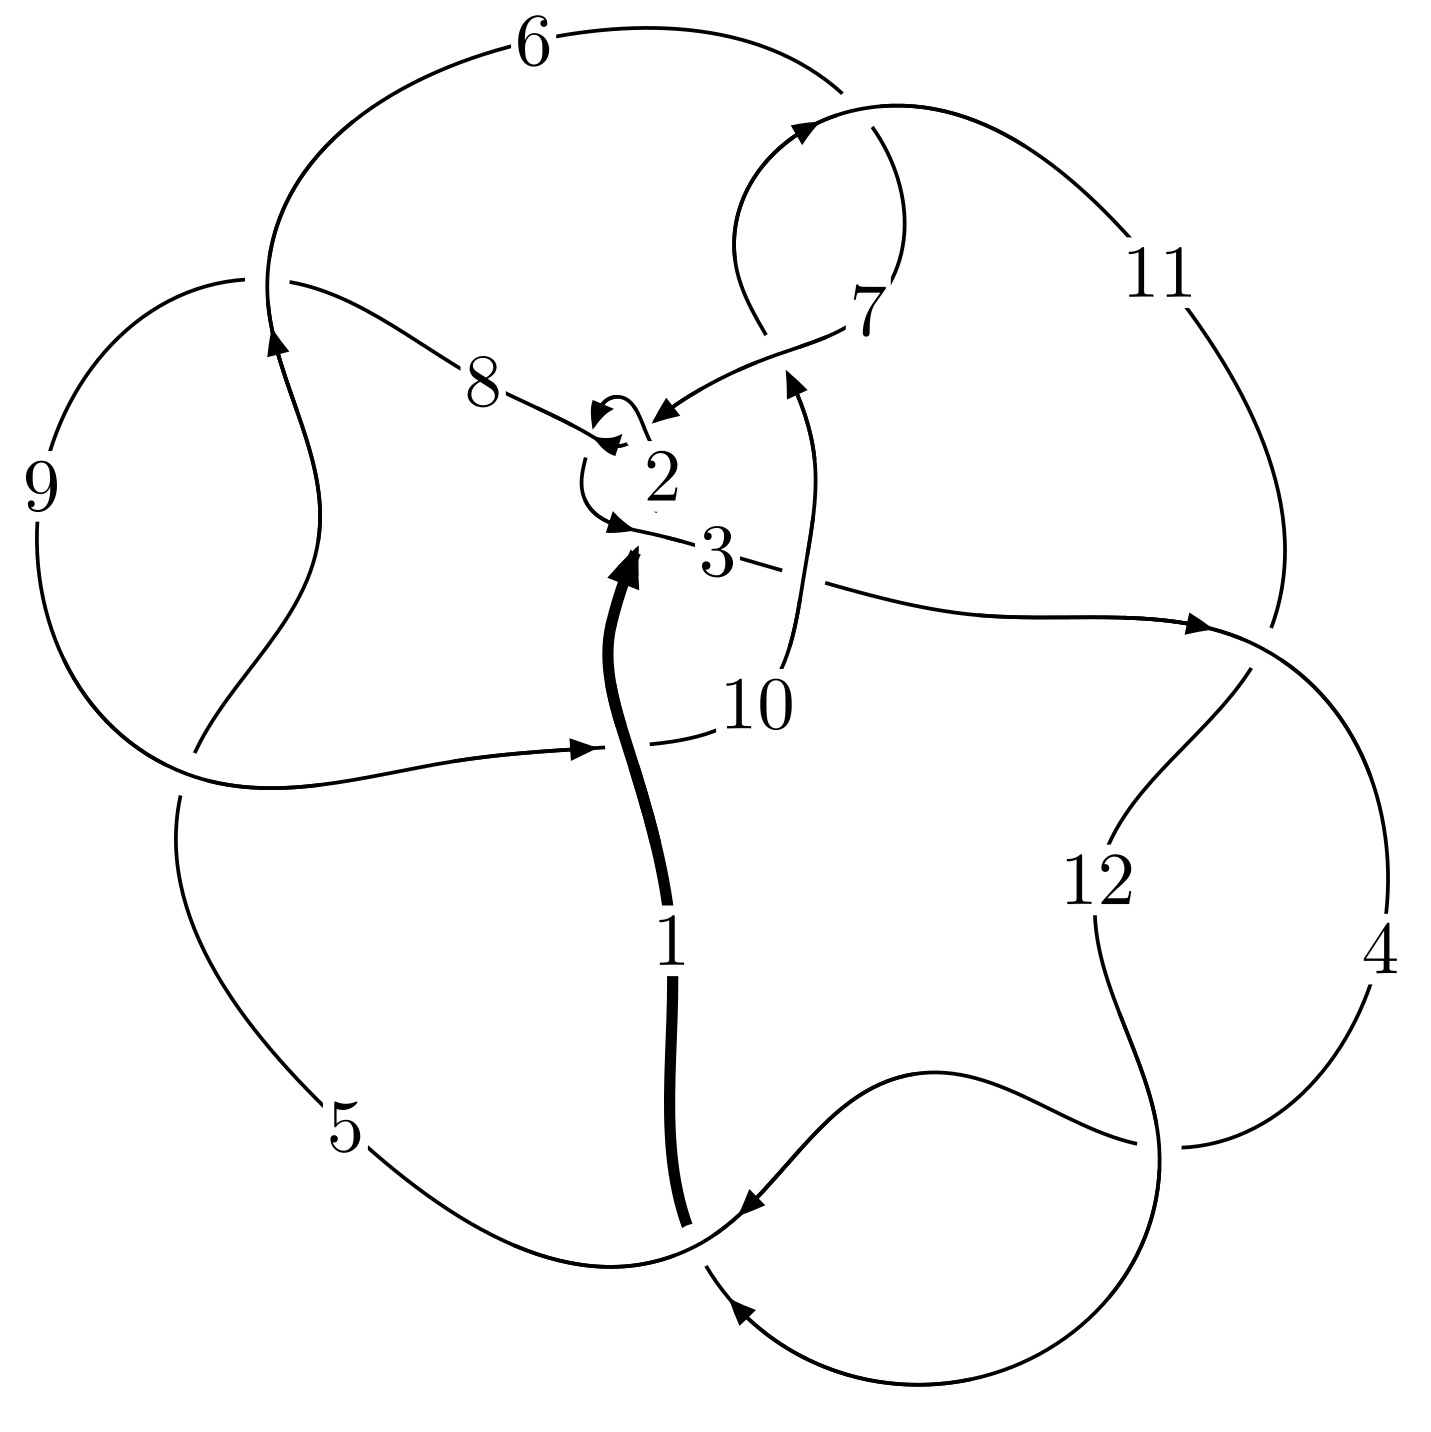
\includegraphics[width=112pt]{../../../GIT/diagram.site/Diagrams/png/1569_12a_0768.png}\\
\ \ \ A knot diagram\footnotemark}&
\allowdisplaybreaks
\textbf{Linearized knot diagam} \\
\cline{2-2}
 &
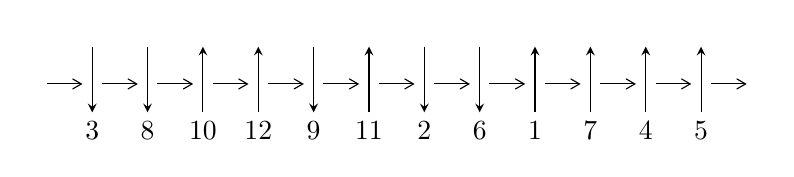
\begin{tikzpicture}[x=20pt, y=17pt]
	% nodes
	\node (C0) at (0, 0) {};
	\node (C1) at (1, 0) {};
	\node (C1U) at (1, +1) {};
	\node (C1D) at (1, -1) {3};

	\node (C2) at (2, 0) {};
	\node (C2U) at (2, +1) {};
	\node (C2D) at (2, -1) {8};

	\node (C3) at (3, 0) {};
	\node (C3U) at (3, +1) {};
	\node (C3D) at (3, -1) {10};

	\node (C4) at (4, 0) {};
	\node (C4U) at (4, +1) {};
	\node (C4D) at (4, -1) {12};

	\node (C5) at (5, 0) {};
	\node (C5U) at (5, +1) {};
	\node (C5D) at (5, -1) {9};

	\node (C6) at (6, 0) {};
	\node (C6U) at (6, +1) {};
	\node (C6D) at (6, -1) {11};

	\node (C7) at (7, 0) {};
	\node (C7U) at (7, +1) {};
	\node (C7D) at (7, -1) {2};

	\node (C8) at (8, 0) {};
	\node (C8U) at (8, +1) {};
	\node (C8D) at (8, -1) {6};

	\node (C9) at (9, 0) {};
	\node (C9U) at (9, +1) {};
	\node (C9D) at (9, -1) {1};

	\node (C10) at (10, 0) {};
	\node (C10U) at (10, +1) {};
	\node (C10D) at (10, -1) {7};

	\node (C11) at (11, 0) {};
	\node (C11U) at (11, +1) {};
	\node (C11D) at (11, -1) {4};

	\node (C12) at (12, 0) {};
	\node (C12U) at (12, +1) {};
	\node (C12D) at (12, -1) {5};
	\node (C13) at (13, 0) {};

	% arrows
	\draw[->,>={angle 60}]
	(C0) edge (C1) (C1) edge (C2) (C2) edge (C3) (C3) edge (C4) (C4) edge (C5) (C5) edge (C6) (C6) edge (C7) (C7) edge (C8) (C8) edge (C9) (C9) edge (C10) (C10) edge (C11) (C11) edge (C12) (C12) edge (C13) ;	\draw[->,>=stealth]
	(C1U) edge (C1D) (C2U) edge (C2D) (C3D) edge (C3U) (C4D) edge (C4U) (C5U) edge (C5D) (C6D) edge (C6U) (C7U) edge (C7D) (C8U) edge (C8D) (C9D) edge (C9U) (C10D) edge (C10U) (C11D) edge (C11U) (C12D) edge (C12U) ;
	\end{tikzpicture} \\
\hhline{~~} \\& 
\textbf{Solving Sequence} \\ \cline{2-2} 
 &
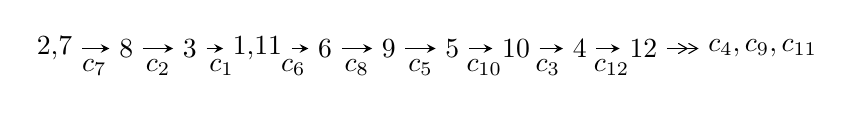
\begin{tikzpicture}[x=23pt, y=7pt]
	% node
	\node (A0) at (-1/8, 0) {2,7};
	\node (A1) at (1, 0) {8};
	\node (A2) at (2, 0) {3};
	\node (A3) at (49/16, 0) {1,11};
	\node (A4) at (33/8, 0) {6};
	\node (A5) at (41/8, 0) {9};
	\node (A6) at (49/8, 0) {5};
	\node (A7) at (57/8, 0) {10};
	\node (A8) at (65/8, 0) {4};
	\node (A9) at (73/8, 0) {12};
	\node (C1) at (1/2, -1) {$c_{7}$};
	\node (C2) at (3/2, -1) {$c_{2}$};
	\node (C3) at (5/2, -1) {$c_{1}$};
	\node (C4) at (29/8, -1) {$c_{6}$};
	\node (C5) at (37/8, -1) {$c_{8}$};
	\node (C6) at (45/8, -1) {$c_{5}$};
	\node (C7) at (53/8, -1) {$c_{10}$};
	\node (C8) at (61/8, -1) {$c_{3}$};
	\node (C9) at (69/8, -1) {$c_{12}$};
	\node (A10) at (11, 0) {$c_{4},c_{9},c_{11}$};

	% edge
	\draw[->,>=stealth]	
	(A0) edge (A1) (A1) edge (A2) (A2) edge (A3) (A3) edge (A4) (A4) edge (A5) (A5) edge (A6) (A6) edge (A7) (A7) edge (A8) (A8) edge (A9) ;
	\draw[->>,>={angle 60}]	
	(A9) edge (A10);
\end{tikzpicture} \\ 

\end{tabular} \\

\footnotetext{
The image of knot diagram is generated by the software ``\textbf{Draw programme}" developed by Andrew Bartholomew(\url{http://www.layer8.co.uk/maths/draw/index.htm\#Running-draw}), where we modified some parts for our purpose(\url{https://github.com/CATsTAILs/LinksPainter}).
}\phantom \\ \newline 
\centering \textbf{Ideals for irreducible components\footnotemark of $X_{\text{par}}$} 
 
\begin{align*}
I^u_{1}&=\langle 
-7.73657\times10^{241} u^{120}+4.38054\times10^{242} u^{119}+\cdots+2.91273\times10^{242} b+6.42953\times10^{244},\\
\phantom{I^u_{1}}&\phantom{= \langle  }-3.27173\times10^{245} u^{120}+6.31064\times10^{244} u^{119}+\cdots+2.82535\times10^{244} a+3.29447\times10^{247},\\
\phantom{I^u_{1}}&\phantom{= \langle  }u^{121}- u^{120}+\cdots+69 u+97\rangle \\
I^u_{2}&=\langle 
4116 u^{29}-337 u^{28}+\cdots+2119 b-4263,\;3524 u^{29}-3466 u^{28}+\cdots+2119 a-4558,\\
\phantom{I^u_{2}}&\phantom{= \langle  }u^{30}-9 u^{28}+\cdots+u+1\rangle \\
\\
\end{align*}
\raggedright * 2 irreducible components of $\dim_{\mathbb{C}}=0$, with total 151 representations.\\
\footnotetext{All coefficients of polynomials are rational numbers. But the coefficients are sometimes approximated in decimal forms when there is not enough margin.}
\newpage
\renewcommand{\arraystretch}{1}
\centering \section*{I. $I^u_{1}= \langle -7.74\times10^{241} u^{120}+4.38\times10^{242} u^{119}+\cdots+2.91\times10^{242} b+6.43\times10^{244},\;-3.27\times10^{245} u^{120}+6.31\times10^{244} u^{119}+\cdots+2.83\times10^{244} a+3.29\times10^{247},\;u^{121}- u^{120}+\cdots+69 u+97 \rangle$}
\flushleft \textbf{(i) Arc colorings}\\
\begin{tabular}{m{7pt} m{180pt} m{7pt} m{180pt} }
\flushright $a_{2}=$&$\begin{pmatrix}0\\u\end{pmatrix}$ \\
\flushright $a_{7}=$&$\begin{pmatrix}1\\0\end{pmatrix}$ \\
\flushright $a_{8}=$&$\begin{pmatrix}1\\u^2\end{pmatrix}$ \\
\flushright $a_{3}=$&$\begin{pmatrix}- u\\- u^3+u\end{pmatrix}$ \\
\flushright $a_{1}=$&$\begin{pmatrix}u^3\\u^5- u^3+u\end{pmatrix}$ \\
\flushright $a_{11}=$&$\begin{pmatrix}11.5799 u^{120}-2.23358 u^{119}+\cdots-1801.60 u-1166.04\\0.265612 u^{120}-1.50393 u^{119}+\cdots-542.124 u-220.739\end{pmatrix}$ \\
\flushright $a_{6}=$&$\begin{pmatrix}1.69838 u^{120}-1.47920 u^{119}+\cdots-589.566 u-269.583\\2.12353 u^{120}+0.809084 u^{119}+\cdots+114.602 u-39.3418\end{pmatrix}$ \\
\flushright $a_{9}=$&$\begin{pmatrix}12.2633 u^{120}-2.76134 u^{119}+\cdots-2025.46 u-1280.53\\1.73056 u^{120}-2.27706 u^{119}+\cdots-906.620 u-425.142\end{pmatrix}$ \\
\flushright $a_{5}=$&$\begin{pmatrix}12.4360 u^{120}+1.22543 u^{119}+\cdots-796.514 u-810.793\\4.89497 u^{120}+0.173831 u^{119}+\cdots-421.051 u-361.017\end{pmatrix}$ \\
\flushright $a_{10}=$&$\begin{pmatrix}11.3143 u^{120}-0.729653 u^{119}+\cdots-1259.47 u-945.303\\0.265612 u^{120}-1.50393 u^{119}+\cdots-542.124 u-220.739\end{pmatrix}$ \\
\flushright $a_{4}=$&$\begin{pmatrix}21.7193 u^{120}-1.04277 u^{119}+\cdots-2277.03 u-1787.84\\4.31254 u^{120}-1.71411 u^{119}+\cdots-913.787 u-535.612\end{pmatrix}$ \\
\flushright $a_{12}=$&$\begin{pmatrix}-21.9248 u^{120}-0.137626 u^{119}+\cdots+1841.17 u+1620.20\\-6.45237 u^{120}+0.992236 u^{119}+\cdots+856.175 u+596.164\end{pmatrix}$\\&\end{tabular}
\flushleft \textbf{(ii) Obstruction class $= -1$}\\~\\
\flushleft \textbf{(iii) Cusp Shapes $= 4.96927 u^{120}-2.45619 u^{119}+\cdots-1122.54 u-555.660$}\\~\\
\newpage\renewcommand{\arraystretch}{1}
\flushleft \textbf{(iv) u-Polynomials at the component}\newline \\
\begin{tabular}{m{50pt}|m{274pt}}
Crossings & \hspace{64pt}u-Polynomials at each crossing \\
\hline $$\begin{aligned}c_{1}\end{aligned}$$&$\begin{aligned}
&u^{121}+55 u^{120}+\cdots+178585 u+9409
\end{aligned}$\\
\hline $$\begin{aligned}c_{2},c_{7}\end{aligned}$$&$\begin{aligned}
&u^{121}+u^{120}+\cdots+69 u-97
\end{aligned}$\\
\hline $$\begin{aligned}c_{3}\end{aligned}$$&$\begin{aligned}
&u^{121}-10 u^{119}+\cdots-165094 u-9137
\end{aligned}$\\
\hline $$\begin{aligned}c_{4},c_{11},c_{12}\end{aligned}$$&$\begin{aligned}
&u^{121}-3 u^{120}+\cdots+5 u-2
\end{aligned}$\\
\hline $$\begin{aligned}c_{5},c_{8}\end{aligned}$$&$\begin{aligned}
&u^{121}-3 u^{120}+\cdots-837975 u+184601
\end{aligned}$\\
\hline $$\begin{aligned}c_{6},c_{10}\end{aligned}$$&$\begin{aligned}
&u^{121}-2 u^{120}+\cdots-1722 u+181
\end{aligned}$\\
\hline $$\begin{aligned}c_{9}\end{aligned}$$&$\begin{aligned}
&u^{121}-7 u^{120}+\cdots-1422961227 u+245450119
\end{aligned}$\\
\hline
\end{tabular}\\~\\
\newpage\renewcommand{\arraystretch}{1}
\flushleft \textbf{(v) Riley Polynomials at the component}\newline \\
\begin{tabular}{m{50pt}|m{274pt}}
Crossings & \hspace{64pt}Riley Polynomials at each crossing \\
\hline $$\begin{aligned}c_{1}\end{aligned}$$&$\begin{aligned}
&y^{121}+37 y^{120}+\cdots-3380797875 y-88529281
\end{aligned}$\\
\hline $$\begin{aligned}c_{2},c_{7}\end{aligned}$$&$\begin{aligned}
&y^{121}-55 y^{120}+\cdots+178585 y-9409
\end{aligned}$\\
\hline $$\begin{aligned}c_{3}\end{aligned}$$&$\begin{aligned}
&y^{121}-20 y^{120}+\cdots+9314834924 y-83484769
\end{aligned}$\\
\hline $$\begin{aligned}c_{4},c_{11},c_{12}\end{aligned}$$&$\begin{aligned}
&y^{121}-127 y^{120}+\cdots-235 y-4
\end{aligned}$\\
\hline $$\begin{aligned}c_{5},c_{8}\end{aligned}$$&$\begin{aligned}
&y^{121}+99 y^{120}+\cdots-1160560440125 y-34077529201
\end{aligned}$\\
\hline $$\begin{aligned}c_{6},c_{10}\end{aligned}$$&$\begin{aligned}
&y^{121}+66 y^{120}+\cdots-951918 y-32761
\end{aligned}$\\
\hline $$\begin{aligned}c_{9}\end{aligned}$$&$\begin{aligned}
&y^{121}-57 y^{120}+\cdots+1931211107502902003 y-60245760917114161
\end{aligned}$\\
\hline
\end{tabular}\\~\\
\newpage\flushleft \textbf{(vi) Complex Volumes and Cusp Shapes}
$$\begin{array}{c|c|c}  
\text{Solutions to }I^u_{1}& \I (\text{vol} + \sqrt{-1}CS) & \text{Cusp shape}\\
 \hline 
\begin{aligned}
u &= -0.876286 + 0.467559 I \\
a &= -1.03412 + 1.96518 I \\
b &= -0.13388 + 1.60777 I\end{aligned}
 & -2.33587 + 1.90742 I & \phantom{-0.000000 } 0 \\ \hline\begin{aligned}
u &= -0.876286 - 0.467559 I \\
a &= -1.03412 - 1.96518 I \\
b &= -0.13388 - 1.60777 I\end{aligned}
 & -2.33587 - 1.90742 I & \phantom{-0.000000 } 0 \\ \hline\begin{aligned}
u &= \phantom{-}0.628684 + 0.789411 I \\
a &= -0.328672 - 0.857919 I \\
b &= \phantom{-}0.991013 - 0.403719 I\end{aligned}
 & \phantom{-}5.65841 + 2.00130 I & \phantom{-0.000000 } 0 \\ \hline\begin{aligned}
u &= \phantom{-}0.628684 - 0.789411 I \\
a &= -0.328672 + 0.857919 I \\
b &= \phantom{-}0.991013 + 0.403719 I\end{aligned}
 & \phantom{-}5.65841 - 2.00130 I & \phantom{-0.000000 } 0 \\ \hline\begin{aligned}
u &= -0.785193 + 0.575255 I \\
a &= \phantom{-}1.09177 + 1.22957 I \\
b &= -0.499932 + 0.920719 I\end{aligned}
 & \phantom{-}9.17779 - 1.78272 I & \phantom{-0.000000 } 0 \\ \hline\begin{aligned}
u &= -0.785193 - 0.575255 I \\
a &= \phantom{-}1.09177 - 1.22957 I \\
b &= -0.499932 - 0.920719 I\end{aligned}
 & \phantom{-}9.17779 + 1.78272 I & \phantom{-0.000000 } 0 \\ \hline\begin{aligned}
u &= \phantom{-}1.028380 + 0.053307 I \\
a &= \phantom{-}0.10666 + 2.50499 I \\
b &= \phantom{-}0.392925 + 1.276220 I\end{aligned}
 & -0.69195 + 4.37118 I & \phantom{-0.000000 } 0 \\ \hline\begin{aligned}
u &= \phantom{-}1.028380 - 0.053307 I \\
a &= \phantom{-}0.10666 - 2.50499 I \\
b &= \phantom{-}0.392925 - 1.276220 I\end{aligned}
 & -0.69195 - 4.37118 I & \phantom{-0.000000 } 0 \\ \hline\begin{aligned}
u &= -0.877621 + 0.409911 I \\
a &= \phantom{-}2.08542 - 1.40668 I \\
b &= -0.130887 - 0.851392 I\end{aligned}
 & \phantom{-}0.040148 - 0.611165 I & \phantom{-0.000000 } 0 \\ \hline\begin{aligned}
u &= -0.877621 - 0.409911 I \\
a &= \phantom{-}2.08542 + 1.40668 I \\
b &= -0.130887 + 0.851392 I\end{aligned}
 & \phantom{-}0.040148 + 0.611165 I & \phantom{-0.000000 } 0\\
 \hline 
 \end{array}$$\newpage$$\begin{array}{c|c|c}  
\text{Solutions to }I^u_{1}& \I (\text{vol} + \sqrt{-1}CS) & \text{Cusp shape}\\
 \hline 
\begin{aligned}
u &= -0.555036 + 0.786400 I \\
a &= -0.562871 + 0.869067 I \\
b &= \phantom{-}1.172490 + 0.545130 I\end{aligned}
 & \phantom{-}12.53200 - 5.36104 I & \phantom{-0.000000 } 0 \\ \hline\begin{aligned}
u &= -0.555036 - 0.786400 I \\
a &= -0.562871 - 0.869067 I \\
b &= \phantom{-}1.172490 - 0.545130 I\end{aligned}
 & \phantom{-}12.53200 + 5.36104 I & \phantom{-0.000000 } 0 \\ \hline\begin{aligned}
u &= \phantom{-}0.382005 + 0.969451 I \\
a &= -0.001280 + 0.709004 I \\
b &= \phantom{-}0.558470 + 1.003670 I\end{aligned}
 & \phantom{-}3.61406 + 1.95058 I & \phantom{-0.000000 } 0 \\ \hline\begin{aligned}
u &= \phantom{-}0.382005 - 0.969451 I \\
a &= -0.001280 - 0.709004 I \\
b &= \phantom{-}0.558470 - 1.003670 I\end{aligned}
 & \phantom{-}3.61406 - 1.95058 I & \phantom{-0.000000 } 0 \\ \hline\begin{aligned}
u &= -0.579250 + 0.762953 I \\
a &= \phantom{-}0.582393 - 0.021569 I \\
b &= -0.482862 + 1.141440 I\end{aligned}
 & \phantom{-}4.58445 - 5.30494 I & \phantom{-0.000000 } 0 \\ \hline\begin{aligned}
u &= -0.579250 - 0.762953 I \\
a &= \phantom{-}0.582393 + 0.021569 I \\
b &= -0.482862 - 1.141440 I\end{aligned}
 & \phantom{-}4.58445 + 5.30494 I & \phantom{-0.000000 } 0 \\ \hline\begin{aligned}
u &= \phantom{-}0.924481 + 0.502615 I \\
a &= \phantom{-}1.39982 + 1.21824 I \\
b &= -0.486699 + 1.149380 I\end{aligned}
 & -1.93253 - 2.60114 I & \phantom{-0.000000 } 0 \\ \hline\begin{aligned}
u &= \phantom{-}0.924481 - 0.502615 I \\
a &= \phantom{-}1.39982 - 1.21824 I \\
b &= -0.486699 - 1.149380 I\end{aligned}
 & -1.93253 + 2.60114 I & \phantom{-0.000000 } 0 \\ \hline\begin{aligned}
u &= \phantom{-}0.461373 + 0.946018 I \\
a &= -0.172847 + 0.415912 I \\
b &= \phantom{-}0.745875 + 1.200540 I\end{aligned}
 & \phantom{-}10.3436 + 12.1376 I & \phantom{-0.000000 } 0 \\ \hline\begin{aligned}
u &= \phantom{-}0.461373 - 0.946018 I \\
a &= -0.172847 - 0.415912 I \\
b &= \phantom{-}0.745875 - 1.200540 I\end{aligned}
 & \phantom{-}10.3436 - 12.1376 I & \phantom{-0.000000 } 0\\
 \hline 
 \end{array}$$\newpage$$\begin{array}{c|c|c}  
\text{Solutions to }I^u_{1}& \I (\text{vol} + \sqrt{-1}CS) & \text{Cusp shape}\\
 \hline 
\begin{aligned}
u &= \phantom{-}0.835820 + 0.434595 I \\
a &= -0.90971 - 1.10559 I \\
b &= -0.66766 - 1.49732 I\end{aligned}
 & \phantom{-}1.34302 + 1.75143 I & \phantom{-0.000000 } 0 \\ \hline\begin{aligned}
u &= \phantom{-}0.835820 - 0.434595 I \\
a &= -0.90971 + 1.10559 I \\
b &= -0.66766 + 1.49732 I\end{aligned}
 & \phantom{-}1.34302 - 1.75143 I & \phantom{-0.000000 } 0 \\ \hline\begin{aligned}
u &= -0.444869 + 0.961457 I \\
a &= -0.067492 - 0.520847 I \\
b &= \phantom{-}0.641967 - 1.142950 I\end{aligned}
 & \phantom{-}3.37355 - 7.82461 I & \phantom{-0.000000 } 0 \\ \hline\begin{aligned}
u &= -0.444869 - 0.961457 I \\
a &= -0.067492 + 0.520847 I \\
b &= \phantom{-}0.641967 + 1.142950 I\end{aligned}
 & \phantom{-}3.37355 + 7.82461 I & \phantom{-0.000000 } 0 \\ \hline\begin{aligned}
u &= \phantom{-}0.952588 + 0.467385 I \\
a &= -1.11573 - 2.35287 I \\
b &= \phantom{-}0.49581 - 1.52570 I\end{aligned}
 & \phantom{-}0.89960 - 5.41363 I & \phantom{-0.000000 } 0 \\ \hline\begin{aligned}
u &= \phantom{-}0.952588 - 0.467385 I \\
a &= -1.11573 + 2.35287 I \\
b &= \phantom{-}0.49581 + 1.52570 I\end{aligned}
 & \phantom{-}0.89960 + 5.41363 I & \phantom{-0.000000 } 0 \\ \hline\begin{aligned}
u &= \phantom{-}0.858991 + 0.373902 I \\
a &= \phantom{-}0.271095 - 0.014070 I \\
b &= \phantom{-}0.501503 + 0.468384 I\end{aligned}
 & -1.31179 - 1.12224 I & \phantom{-0.000000 } 0 \\ \hline\begin{aligned}
u &= \phantom{-}0.858991 - 0.373902 I \\
a &= \phantom{-}0.271095 + 0.014070 I \\
b &= \phantom{-}0.501503 - 0.468384 I\end{aligned}
 & -1.31179 + 1.12224 I & \phantom{-0.000000 } 0 \\ \hline\begin{aligned}
u &= -0.934802\phantom{ +0.000000I} \\
a &= \phantom{-}0.887196\phantom{ +0.000000I} \\
b &= \phantom{-}0.823832\phantom{ +0.000000I}\end{aligned}
 & \phantom{-}3.31166\phantom{ +0.000000I} & \phantom{-0.000000 } 0 \\ \hline\begin{aligned}
u &= -0.907481 + 0.567494 I \\
a &= -1.55067 + 2.95784 I \\
b &= \phantom{-}0.318129 + 0.986288 I\end{aligned}
 & \phantom{-}8.78876 + 6.33873 I & \phantom{-0.000000 } 0\\
 \hline 
 \end{array}$$\newpage$$\begin{array}{c|c|c}  
\text{Solutions to }I^u_{1}& \I (\text{vol} + \sqrt{-1}CS) & \text{Cusp shape}\\
 \hline 
\begin{aligned}
u &= -0.907481 - 0.567494 I \\
a &= -1.55067 - 2.95784 I \\
b &= \phantom{-}0.318129 - 0.986288 I\end{aligned}
 & \phantom{-}8.78876 - 6.33873 I & \phantom{-0.000000 } 0 \\ \hline\begin{aligned}
u &= -0.958093 + 0.481293 I \\
a &= -0.349548 + 0.404271 I \\
b &= \phantom{-}0.535148 - 0.271890 I\end{aligned}
 & -0.45371 + 4.02618 I & \phantom{-0.000000 } 0 \\ \hline\begin{aligned}
u &= -0.958093 - 0.481293 I \\
a &= -0.349548 - 0.404271 I \\
b &= \phantom{-}0.535148 + 0.271890 I\end{aligned}
 & -0.45371 - 4.02618 I & \phantom{-0.000000 } 0 \\ \hline\begin{aligned}
u &= \phantom{-}0.927649 + 0.017401 I \\
a &= -0.311560 - 1.244890 I \\
b &= -0.887556 + 0.155488 I\end{aligned}
 & \phantom{-}6.96948 - 4.64303 I & \phantom{-0.000000 } 0 \\ \hline\begin{aligned}
u &= \phantom{-}0.927649 - 0.017401 I \\
a &= -0.311560 + 1.244890 I \\
b &= -0.887556 - 0.155488 I\end{aligned}
 & \phantom{-}6.96948 + 4.64303 I & \phantom{-0.000000 } 0 \\ \hline\begin{aligned}
u &= \phantom{-}0.941684 + 0.514503 I \\
a &= -1.18628 - 2.38991 I \\
b &= \phantom{-}0.386899 - 1.296100 I\end{aligned}
 & \phantom{-}0.79803 - 5.41123 I & \phantom{-0.000000 } 0 \\ \hline\begin{aligned}
u &= \phantom{-}0.941684 - 0.514503 I \\
a &= -1.18628 + 2.38991 I \\
b &= \phantom{-}0.386899 + 1.296100 I\end{aligned}
 & \phantom{-}0.79803 + 5.41123 I & \phantom{-0.000000 } 0 \\ \hline\begin{aligned}
u &= -0.921007 + 0.557173 I \\
a &= \phantom{-}1.00367 - 1.24207 I \\
b &= -0.92522 - 1.12569 I\end{aligned}
 & \phantom{-}2.32592 + 5.93979 I & \phantom{-0.000000 } 0 \\ \hline\begin{aligned}
u &= -0.921007 - 0.557173 I \\
a &= \phantom{-}1.00367 + 1.24207 I \\
b &= -0.92522 + 1.12569 I\end{aligned}
 & \phantom{-}2.32592 - 5.93979 I & \phantom{-0.000000 } 0 \\ \hline\begin{aligned}
u &= -0.350745 + 0.852172 I \\
a &= -0.104211 - 1.025600 I \\
b &= \phantom{-}0.630751 - 0.791397 I\end{aligned}
 & \phantom{-}11.40380 + 2.13821 I & \phantom{-0.000000 } 0\\
 \hline 
 \end{array}$$\newpage$$\begin{array}{c|c|c}  
\text{Solutions to }I^u_{1}& \I (\text{vol} + \sqrt{-1}CS) & \text{Cusp shape}\\
 \hline 
\begin{aligned}
u &= -0.350745 - 0.852172 I \\
a &= -0.104211 + 1.025600 I \\
b &= \phantom{-}0.630751 + 0.791397 I\end{aligned}
 & \phantom{-}11.40380 - 2.13821 I & \phantom{-0.000000 } 0 \\ \hline\begin{aligned}
u &= -0.719109 + 0.574145 I \\
a &= \phantom{-}0.691803 + 0.523675 I \\
b &= \phantom{-}0.757134 - 0.858710 I\end{aligned}
 & \phantom{-}2.91905 - 1.41856 I & \phantom{-0.000000 } 0 \\ \hline\begin{aligned}
u &= -0.719109 - 0.574145 I \\
a &= \phantom{-}0.691803 - 0.523675 I \\
b &= \phantom{-}0.757134 + 0.858710 I\end{aligned}
 & \phantom{-}2.91905 + 1.41856 I & \phantom{-0.000000 } 0 \\ \hline\begin{aligned}
u &= \phantom{-}0.830251 + 0.391156 I \\
a &= \phantom{-}3.38644 + 1.37950 I \\
b &= -0.055557 + 0.599876 I\end{aligned}
 & \phantom{-}7.60785 + 2.16745 I & \phantom{-0.000000 } 0 \\ \hline\begin{aligned}
u &= \phantom{-}0.830251 - 0.391156 I \\
a &= \phantom{-}3.38644 - 1.37950 I \\
b &= -0.055557 - 0.599876 I\end{aligned}
 & \phantom{-}7.60785 - 2.16745 I & \phantom{-0.000000 } 0 \\ \hline\begin{aligned}
u &= \phantom{-}0.479627 + 0.742494 I \\
a &= \phantom{-}0.522768 - 0.104455 I \\
b &= -0.368163 - 1.001770 I\end{aligned}
 & -1.11708 + 2.95125 I & \phantom{-0.000000 } 0 \\ \hline\begin{aligned}
u &= \phantom{-}0.479627 - 0.742494 I \\
a &= \phantom{-}0.522768 + 0.104455 I \\
b &= -0.368163 + 1.001770 I\end{aligned}
 & -1.11708 - 2.95125 I & \phantom{-0.000000 } 0 \\ \hline\begin{aligned}
u &= \phantom{-}1.070760 + 0.334175 I \\
a &= \phantom{-}1.11644 + 1.32522 I \\
b &= \phantom{-}0.443247 + 1.239720 I\end{aligned}
 & -2.93291 - 0.35986 I & \phantom{-0.000000 } 0 \\ \hline\begin{aligned}
u &= \phantom{-}1.070760 - 0.334175 I \\
a &= \phantom{-}1.11644 - 1.32522 I \\
b &= \phantom{-}0.443247 - 1.239720 I\end{aligned}
 & -2.93291 + 0.35986 I & \phantom{-0.000000 } 0 \\ \hline\begin{aligned}
u &= \phantom{-}0.728022 + 0.482499 I \\
a &= \phantom{-}0.175720 - 0.731462 I \\
b &= -0.616716 - 1.057780 I\end{aligned}
 & \phantom{-}1.51362 + 1.28957 I & \phantom{-0.000000 } 0\\
 \hline 
 \end{array}$$\newpage$$\begin{array}{c|c|c}  
\text{Solutions to }I^u_{1}& \I (\text{vol} + \sqrt{-1}CS) & \text{Cusp shape}\\
 \hline 
\begin{aligned}
u &= \phantom{-}0.728022 - 0.482499 I \\
a &= \phantom{-}0.175720 + 0.731462 I \\
b &= -0.616716 + 1.057780 I\end{aligned}
 & \phantom{-}1.51362 - 1.28957 I & \phantom{-0.000000 } 0 \\ \hline\begin{aligned}
u &= -1.126030 + 0.136649 I \\
a &= \phantom{-}0.11797 - 2.12973 I \\
b &= \phantom{-}0.177424 - 1.214160 I\end{aligned}
 & -6.09582 - 1.01611 I & \phantom{-0.000000 } 0 \\ \hline\begin{aligned}
u &= -1.126030 - 0.136649 I \\
a &= \phantom{-}0.11797 + 2.12973 I \\
b &= \phantom{-}0.177424 + 1.214160 I\end{aligned}
 & -6.09582 + 1.01611 I & \phantom{-0.000000 } 0 \\ \hline\begin{aligned}
u &= \phantom{-}0.837251 + 0.770716 I \\
a &= \phantom{-}0.695837 - 0.221942 I \\
b &= -0.454504 + 0.782523 I\end{aligned}
 & \phantom{-}9.66264 - 2.15233 I & \phantom{-0.000000 } 0 \\ \hline\begin{aligned}
u &= \phantom{-}0.837251 - 0.770716 I \\
a &= \phantom{-}0.695837 + 0.221942 I \\
b &= -0.454504 - 0.782523 I\end{aligned}
 & \phantom{-}9.66264 + 2.15233 I & \phantom{-0.000000 } 0 \\ \hline\begin{aligned}
u &= -0.707677 + 0.891972 I \\
a &= -0.193028 + 0.625350 I \\
b &= \phantom{-}0.581995 + 0.488567 I\end{aligned}
 & \phantom{-}5.07524 + 2.65277 I & \phantom{-0.000000 } 0 \\ \hline\begin{aligned}
u &= -0.707677 - 0.891972 I \\
a &= -0.193028 - 0.625350 I \\
b &= \phantom{-}0.581995 - 0.488567 I\end{aligned}
 & \phantom{-}5.07524 - 2.65277 I & \phantom{-0.000000 } 0 \\ \hline\begin{aligned}
u &= -1.057440 + 0.426765 I \\
a &= \phantom{-}1.37614 - 1.42332 I \\
b &= \phantom{-}0.11276 - 1.50273 I\end{aligned}
 & \phantom{-}0.959736 + 0.654295 I & \phantom{-0.000000 } 0 \\ \hline\begin{aligned}
u &= -1.057440 - 0.426765 I \\
a &= \phantom{-}1.37614 + 1.42332 I \\
b &= \phantom{-}0.11276 + 1.50273 I\end{aligned}
 & \phantom{-}0.959736 - 0.654295 I & \phantom{-0.000000 } 0 \\ \hline\begin{aligned}
u &= \phantom{-}0.611340 + 0.968423 I \\
a &= -0.259712 - 0.474871 I \\
b &= \phantom{-}0.587643 - 0.851228 I\end{aligned}
 & \phantom{-}11.23210 - 6.90153 I & \phantom{-0.000000 } 0\\
 \hline 
 \end{array}$$\newpage$$\begin{array}{c|c|c}  
\text{Solutions to }I^u_{1}& \I (\text{vol} + \sqrt{-1}CS) & \text{Cusp shape}\\
 \hline 
\begin{aligned}
u &= \phantom{-}0.611340 - 0.968423 I \\
a &= -0.259712 + 0.474871 I \\
b &= \phantom{-}0.587643 + 0.851228 I\end{aligned}
 & \phantom{-}11.23210 + 6.90153 I & \phantom{-0.000000 } 0 \\ \hline\begin{aligned}
u &= \phantom{-}1.091290 + 0.353150 I \\
a &= -1.04122 - 1.67611 I \\
b &= -0.123169 - 0.278771 I\end{aligned}
 & \phantom{-}6.85939 - 5.07145 I & \phantom{-0.000000 } 0 \\ \hline\begin{aligned}
u &= \phantom{-}1.091290 - 0.353150 I \\
a &= -1.04122 + 1.67611 I \\
b &= -0.123169 + 0.278771 I\end{aligned}
 & \phantom{-}6.85939 + 5.07145 I & \phantom{-0.000000 } 0 \\ \hline\begin{aligned}
u &= \phantom{-}1.009210 + 0.564259 I \\
a &= -0.250923 - 1.008240 I \\
b &= \phantom{-}0.853707 + 0.108289 I\end{aligned}
 & \phantom{-}6.25063 - 5.57396 I & \phantom{-0.000000 } 0 \\ \hline\begin{aligned}
u &= \phantom{-}1.009210 - 0.564259 I \\
a &= -0.250923 + 1.008240 I \\
b &= \phantom{-}0.853707 - 0.108289 I\end{aligned}
 & \phantom{-}6.25063 + 5.57396 I & \phantom{-0.000000 } 0 \\ \hline\begin{aligned}
u &= -1.115600 + 0.304284 I \\
a &= \phantom{-}1.20339 - 1.05375 I \\
b &= \phantom{-}0.75678 - 1.26996 I\end{aligned}
 & \phantom{-}2.24449 - 0.21390 I & \phantom{-0.000000 } 0 \\ \hline\begin{aligned}
u &= -1.115600 - 0.304284 I \\
a &= \phantom{-}1.20339 + 1.05375 I \\
b &= \phantom{-}0.75678 + 1.26996 I\end{aligned}
 & \phantom{-}2.24449 + 0.21390 I & \phantom{-0.000000 } 0 \\ \hline\begin{aligned}
u &= -0.878670 + 0.772323 I \\
a &= \phantom{-}0.361367 + 0.400725 I \\
b &= -0.039707 - 0.474456 I\end{aligned}
 & \phantom{-}4.22761 + 2.91062 I & \phantom{-0.000000 } 0 \\ \hline\begin{aligned}
u &= -0.878670 - 0.772323 I \\
a &= \phantom{-}0.361367 - 0.400725 I \\
b &= -0.039707 + 0.474456 I\end{aligned}
 & \phantom{-}4.22761 - 2.91062 I & \phantom{-0.000000 } 0 \\ \hline\begin{aligned}
u &= -0.270783 + 0.776768 I \\
a &= \phantom{-}0.551880 + 0.363525 I \\
b &= -0.092386 + 0.752153 I\end{aligned}
 & \phantom{-}0.646581 + 0.057662 I & \phantom{-0.000000 } 0\\
 \hline 
 \end{array}$$\newpage$$\begin{array}{c|c|c}  
\text{Solutions to }I^u_{1}& \I (\text{vol} + \sqrt{-1}CS) & \text{Cusp shape}\\
 \hline 
\begin{aligned}
u &= -0.270783 - 0.776768 I \\
a &= \phantom{-}0.551880 - 0.363525 I \\
b &= -0.092386 - 0.752153 I\end{aligned}
 & \phantom{-}0.646581 - 0.057662 I & \phantom{-0.000000 } 0 \\ \hline\begin{aligned}
u &= -1.062840 + 0.508012 I \\
a &= -0.88319 + 1.97356 I \\
b &= \phantom{-}0.86053 + 1.13805 I\end{aligned}
 & -1.81072 + 6.57692 I & \phantom{-0.000000 } 0 \\ \hline\begin{aligned}
u &= -1.062840 - 0.508012 I \\
a &= -0.88319 - 1.97356 I \\
b &= \phantom{-}0.86053 - 1.13805 I\end{aligned}
 & -1.81072 - 6.57692 I & \phantom{-0.000000 } 0 \\ \hline\begin{aligned}
u &= \phantom{-}0.898488 + 0.772325 I \\
a &= \phantom{-}0.484655 - 0.655901 I \\
b &= \phantom{-}0.301800 + 0.793066 I\end{aligned}
 & \phantom{-}9.49179 - 3.65525 I & \phantom{-0.000000 } 0 \\ \hline\begin{aligned}
u &= \phantom{-}0.898488 - 0.772325 I \\
a &= \phantom{-}0.484655 + 0.655901 I \\
b &= \phantom{-}0.301800 - 0.793066 I\end{aligned}
 & \phantom{-}9.49179 + 3.65525 I & \phantom{-0.000000 } 0 \\ \hline\begin{aligned}
u &= \phantom{-}0.479958 + 0.637359 I \\
a &= \phantom{-}0.992882 - 0.043182 I \\
b &= -0.828420 + 0.013782 I\end{aligned}
 & \phantom{-}7.76200 + 0.90081 I & \phantom{-0.000000 } 0 \\ \hline\begin{aligned}
u &= \phantom{-}0.479958 - 0.637359 I \\
a &= \phantom{-}0.992882 + 0.043182 I \\
b &= -0.828420 - 0.013782 I\end{aligned}
 & \phantom{-}7.76200 - 0.90081 I & \phantom{-0.000000 } 0 \\ \hline\begin{aligned}
u &= \phantom{-}1.102970 + 0.503764 I \\
a &= -0.63027 - 1.96483 I \\
b &= \phantom{-}1.14012 - 1.07707 I\end{aligned}
 & \phantom{-}3.51683 - 7.73270 I & \phantom{-0.000000 } 0 \\ \hline\begin{aligned}
u &= \phantom{-}1.102970 - 0.503764 I \\
a &= -0.63027 + 1.96483 I \\
b &= \phantom{-}1.14012 + 1.07707 I\end{aligned}
 & \phantom{-}3.51683 + 7.73270 I & \phantom{-0.000000 } 0 \\ \hline\begin{aligned}
u &= -0.967783 + 0.734001 I \\
a &= -0.0906118 - 0.0915978 I \\
b &= -0.649807 + 0.075200 I\end{aligned}
 & \phantom{-}4.26830 + 3.31666 I & \phantom{-0.000000 } 0\\
 \hline 
 \end{array}$$\newpage$$\begin{array}{c|c|c}  
\text{Solutions to }I^u_{1}& \I (\text{vol} + \sqrt{-1}CS) & \text{Cusp shape}\\
 \hline 
\begin{aligned}
u &= -0.967783 - 0.734001 I \\
a &= -0.0906118 + 0.0915978 I \\
b &= -0.649807 - 0.075200 I\end{aligned}
 & \phantom{-}4.26830 - 3.31666 I & \phantom{-0.000000 } 0 \\ \hline\begin{aligned}
u &= \phantom{-}1.017900 + 0.664460 I \\
a &= -0.402680 + 0.502405 I \\
b &= -1.167080 - 0.230589 I\end{aligned}
 & \phantom{-}4.46966 - 7.47764 I & \phantom{-0.000000 } 0 \\ \hline\begin{aligned}
u &= \phantom{-}1.017900 - 0.664460 I \\
a &= -0.402680 - 0.502405 I \\
b &= -1.167080 + 0.230589 I\end{aligned}
 & \phantom{-}4.46966 + 7.47764 I & \phantom{-0.000000 } 0 \\ \hline\begin{aligned}
u &= -1.045940 + 0.653890 I \\
a &= -1.64671 + 1.40041 I \\
b &= \phantom{-}0.558259 + 1.194000 I\end{aligned}
 & \phantom{-}3.18345 + 10.69620 I & \phantom{-0.000000 } 0 \\ \hline\begin{aligned}
u &= -1.045940 - 0.653890 I \\
a &= -1.64671 - 1.40041 I \\
b &= \phantom{-}0.558259 - 1.194000 I\end{aligned}
 & \phantom{-}3.18345 - 10.69620 I & \phantom{-0.000000 } 0 \\ \hline\begin{aligned}
u &= -1.053880 + 0.647496 I \\
a &= -0.663406 - 0.555628 I \\
b &= -1.34657 + 0.45968 I\end{aligned}
 & \phantom{-}11.0303 + 10.7709 I & \phantom{-0.000000 } 0 \\ \hline\begin{aligned}
u &= -1.053880 - 0.647496 I \\
a &= -0.663406 + 0.555628 I \\
b &= -1.34657 - 0.45968 I\end{aligned}
 & \phantom{-}11.0303 - 10.7709 I & \phantom{-0.000000 } 0 \\ \hline\begin{aligned}
u &= \phantom{-}1.076090 + 0.621431 I \\
a &= -1.39040 - 1.41475 I \\
b &= \phantom{-}0.480219 - 1.111950 I\end{aligned}
 & -2.86776 - 8.16498 I & \phantom{-0.000000 } 0 \\ \hline\begin{aligned}
u &= \phantom{-}1.076090 - 0.621431 I \\
a &= -1.39040 + 1.41475 I \\
b &= \phantom{-}0.480219 + 1.111950 I\end{aligned}
 & -2.86776 + 8.16498 I & \phantom{-0.000000 } 0 \\ \hline\begin{aligned}
u &= -1.129880 + 0.567356 I \\
a &= -1.04797 + 1.34145 I \\
b &= \phantom{-}0.364899 + 0.870060 I\end{aligned}
 & -1.82164 + 4.93277 I & \phantom{-0.000000 } 0\\
 \hline 
 \end{array}$$\newpage$$\begin{array}{c|c|c}  
\text{Solutions to }I^u_{1}& \I (\text{vol} + \sqrt{-1}CS) & \text{Cusp shape}\\
 \hline 
\begin{aligned}
u &= -1.129880 - 0.567356 I \\
a &= -1.04797 - 1.34145 I \\
b &= \phantom{-}0.364899 - 0.870060 I\end{aligned}
 & -1.82164 - 4.93277 I & \phantom{-0.000000 } 0 \\ \hline\begin{aligned}
u &= \phantom{-}1.248140 + 0.268138 I \\
a &= \phantom{-}0.04522 + 1.80547 I \\
b &= -0.019964 + 1.054360 I\end{aligned}
 & -4.02260 - 3.43535 I & \phantom{-0.000000 } 0 \\ \hline\begin{aligned}
u &= \phantom{-}1.248140 - 0.268138 I \\
a &= \phantom{-}0.04522 - 1.80547 I \\
b &= -0.019964 - 1.054360 I\end{aligned}
 & -4.02260 + 3.43535 I & \phantom{-0.000000 } 0 \\ \hline\begin{aligned}
u &= \phantom{-}0.180834 + 0.663314 I \\
a &= \phantom{-}0.713938 + 0.212808 I \\
b &= -0.900032 - 0.977689 I\end{aligned}
 & \phantom{-}6.04567 + 3.35460 I & \phantom{-}7.97311 - 2.93910 I \\ \hline\begin{aligned}
u &= \phantom{-}0.180834 - 0.663314 I \\
a &= \phantom{-}0.713938 - 0.212808 I \\
b &= -0.900032 + 0.977689 I\end{aligned}
 & \phantom{-}6.04567 - 3.35460 I & \phantom{-}7.97311 + 2.93910 I \\ \hline\begin{aligned}
u &= -1.320090 + 0.033310 I \\
a &= -0.51815 + 1.76906 I \\
b &= -0.532315 + 1.158000 I\end{aligned}
 & \phantom{-}3.75464 - 9.26467 I & \phantom{-0.000000 } 0 \\ \hline\begin{aligned}
u &= -1.320090 - 0.033310 I \\
a &= -0.51815 - 1.76906 I \\
b &= -0.532315 - 1.158000 I\end{aligned}
 & \phantom{-}3.75464 + 9.26467 I & \phantom{-0.000000 } 0 \\ \hline\begin{aligned}
u &= -0.676066 + 0.065814 I \\
a &= \phantom{-}0.077833 - 0.593841 I \\
b &= -0.737152 + 0.602808 I\end{aligned}
 & \phantom{-}0.40459 - 2.77385 I & -0.59107 + 8.95739 I \\ \hline\begin{aligned}
u &= -0.676066 - 0.065814 I \\
a &= \phantom{-}0.077833 + 0.593841 I \\
b &= -0.737152 - 0.602808 I\end{aligned}
 & \phantom{-}0.40459 + 2.77385 I & -0.59107 - 8.95739 I \\ \hline\begin{aligned}
u &= -1.182310 + 0.615283 I \\
a &= \phantom{-}0.56765 - 1.99322 I \\
b &= -0.464189 - 0.971569 I\end{aligned}
 & \phantom{-}8.90211 + 3.33620 I & \phantom{-0.000000 } 0\\
 \hline 
 \end{array}$$\newpage$$\begin{array}{c|c|c}  
\text{Solutions to }I^u_{1}& \I (\text{vol} + \sqrt{-1}CS) & \text{Cusp shape}\\
 \hline 
\begin{aligned}
u &= -1.182310 - 0.615283 I \\
a &= \phantom{-}0.56765 + 1.99322 I \\
b &= -0.464189 + 0.971569 I\end{aligned}
 & \phantom{-}8.90211 - 3.33620 I & \phantom{-0.000000 } 0 \\ \hline\begin{aligned}
u &= \phantom{-}1.148350 + 0.678606 I \\
a &= \phantom{-}1.01782 + 1.85825 I \\
b &= -0.76414 + 1.29683 I\end{aligned}
 & \phantom{-}8.2367 - 18.0724 I & \phantom{-0.000000 } 0 \\ \hline\begin{aligned}
u &= \phantom{-}1.148350 - 0.678606 I \\
a &= \phantom{-}1.01782 - 1.85825 I \\
b &= -0.76414 - 1.29683 I\end{aligned}
 & \phantom{-}8.2367 + 18.0724 I & \phantom{-0.000000 } 0 \\ \hline\begin{aligned}
u &= -1.155810 + 0.679707 I \\
a &= \phantom{-}0.93692 - 1.81046 I \\
b &= -0.64751 - 1.27762 I\end{aligned}
 & \phantom{-}1.19708 + 13.79540 I & \phantom{-0.000000 } 0 \\ \hline\begin{aligned}
u &= -1.155810 - 0.679707 I \\
a &= \phantom{-}0.93692 + 1.81046 I \\
b &= -0.64751 + 1.27762 I\end{aligned}
 & \phantom{-}1.19708 - 13.79540 I & \phantom{-0.000000 } 0 \\ \hline\begin{aligned}
u &= \phantom{-}0.498086 + 0.428072 I \\
a &= \phantom{-}0.626722 - 0.268822 I \\
b &= \phantom{-}0.052856 + 0.818326 I\end{aligned}
 & -1.03941 - 1.27491 I & -0.72097 + 4.37315 I \\ \hline\begin{aligned}
u &= \phantom{-}0.498086 - 0.428072 I \\
a &= \phantom{-}0.626722 + 0.268822 I \\
b &= \phantom{-}0.052856 - 0.818326 I\end{aligned}
 & -1.03941 + 1.27491 I & -0.72097 - 4.37315 I \\ \hline\begin{aligned}
u &= -0.255396 + 0.597292 I \\
a &= \phantom{-}0.555457 + 0.283608 I \\
b &= -0.241429 - 1.252780 I\end{aligned}
 & \phantom{-}3.30691 + 3.23521 I & \phantom{-}6.24553 - 3.44821 I \\ \hline\begin{aligned}
u &= -0.255396 - 0.597292 I \\
a &= \phantom{-}0.555457 - 0.283608 I \\
b &= -0.241429 + 1.252780 I\end{aligned}
 & \phantom{-}3.30691 - 3.23521 I & \phantom{-}6.24553 + 3.44821 I \\ \hline\begin{aligned}
u &= \phantom{-}1.093860 + 0.795677 I \\
a &= -0.568436 - 0.262743 I \\
b &= -0.461055 - 0.707837 I\end{aligned}
 & \phantom{-}9.78375 + 0.50006 I & \phantom{-0.000000 } 0\\
 \hline 
 \end{array}$$\newpage$$\begin{array}{c|c|c}  
\text{Solutions to }I^u_{1}& \I (\text{vol} + \sqrt{-1}CS) & \text{Cusp shape}\\
 \hline 
\begin{aligned}
u &= \phantom{-}1.093860 - 0.795677 I \\
a &= -0.568436 + 0.262743 I \\
b &= -0.461055 + 0.707837 I\end{aligned}
 & \phantom{-}9.78375 - 0.50006 I & \phantom{-0.000000 } 0 \\ \hline\begin{aligned}
u &= \phantom{-}1.177980 + 0.674350 I \\
a &= \phantom{-}0.78139 + 1.79731 I \\
b &= -0.521615 + 1.186440 I\end{aligned}
 & \phantom{-}1.21192 - 7.91472 I & \phantom{-0.000000 } 0 \\ \hline\begin{aligned}
u &= \phantom{-}1.177980 - 0.674350 I \\
a &= \phantom{-}0.78139 - 1.79731 I \\
b &= -0.521615 - 1.186440 I\end{aligned}
 & \phantom{-}1.21192 + 7.91472 I & \phantom{-0.000000 } 0 \\ \hline\begin{aligned}
u &= \phantom{-}1.393250 + 0.062804 I \\
a &= -0.43332 - 1.64211 I \\
b &= -0.361309 - 1.025480 I\end{aligned}
 & -3.28842 + 4.58134 I & \phantom{-0.000000 } 0 \\ \hline\begin{aligned}
u &= \phantom{-}1.393250 - 0.062804 I \\
a &= -0.43332 + 1.64211 I \\
b &= -0.361309 + 1.025480 I\end{aligned}
 & -3.28842 - 4.58134 I & \phantom{-0.000000 } 0 \\ \hline\begin{aligned}
u &= -0.364523 + 0.453468 I \\
a &= \phantom{-}0.949005 + 0.189231 I \\
b &= -0.296430 + 0.043240 I\end{aligned}
 & \phantom{-}1.074570 - 0.364625 I & \phantom{-}8.86158 + 1.00666 I \\ \hline\begin{aligned}
u &= -0.364523 - 0.453468 I \\
a &= \phantom{-}0.949005 - 0.189231 I \\
b &= -0.296430 - 0.043240 I\end{aligned}
 & \phantom{-}1.074570 + 0.364625 I & \phantom{-}8.86158 - 1.00666 I \\ \hline\begin{aligned}
u &= -1.40693 + 0.26293 I \\
a &= -0.54852 + 1.45067 I \\
b &= -0.250889 + 0.828979 I\end{aligned}
 & -2.35349 + 2.05269 I & \phantom{-0.000000 } 0 \\ \hline\begin{aligned}
u &= -1.40693 - 0.26293 I \\
a &= -0.54852 - 1.45067 I \\
b &= -0.250889 - 0.828979 I\end{aligned}
 & -2.35349 - 2.05269 I & \phantom{-0.000000 } 0 \\ \hline\begin{aligned}
u &= -0.195571 + 0.479240 I \\
a &= \phantom{-}0.577297 - 0.172202 I \\
b &= -0.657463 + 0.925136 I\end{aligned}
 & \phantom{-}0.29761 - 2.48770 I & \phantom{-}0.48068 + 5.85360 I\\
 \hline 
 \end{array}$$\newpage$$\begin{array}{c|c|c}  
\text{Solutions to }I^u_{1}& \I (\text{vol} + \sqrt{-1}CS) & \text{Cusp shape}\\
 \hline 
\begin{aligned}
u &= -0.195571 - 0.479240 I \\
a &= \phantom{-}0.577297 + 0.172202 I \\
b &= -0.657463 - 0.925136 I\end{aligned}
 & \phantom{-}0.29761 + 2.48770 I & \phantom{-}0.48068 - 5.85360 I\\
 \hline 
 \end{array}$$\newpage\newpage\renewcommand{\arraystretch}{1}
\centering \section*{II. $I^u_{2}= \langle 4116 u^{29}-337 u^{28}+\cdots+2119 b-4263,\;3524 u^{29}-3466 u^{28}+\cdots+2119 a-4558,\;u^{30}-9 u^{28}+\cdots+u+1 \rangle$}
\flushleft \textbf{(i) Arc colorings}\\
\begin{tabular}{m{7pt} m{180pt} m{7pt} m{180pt} }
\flushright $a_{2}=$&$\begin{pmatrix}0\\u\end{pmatrix}$ \\
\flushright $a_{7}=$&$\begin{pmatrix}1\\0\end{pmatrix}$ \\
\flushright $a_{8}=$&$\begin{pmatrix}1\\u^2\end{pmatrix}$ \\
\flushright $a_{3}=$&$\begin{pmatrix}- u\\- u^3+u\end{pmatrix}$ \\
\flushright $a_{1}=$&$\begin{pmatrix}u^3\\u^5- u^3+u\end{pmatrix}$ \\
\flushright $a_{11}=$&$\begin{pmatrix}-1.66305 u^{29}+1.63568 u^{28}+\cdots+2.02171 u+2.15101\\-1.94243 u^{29}+0.159037 u^{28}+\cdots+2.34545 u+2.01180\end{pmatrix}$ \\
\flushright $a_{6}=$&$\begin{pmatrix}-4.72062 u^{29}+1.47664 u^{28}+\cdots+4.67626 u-0.860783\\-0.183577 u^{29}+0.615857 u^{28}+\cdots+0.898537 u-4.48844\end{pmatrix}$ \\
\flushright $a_{9}=$&$\begin{pmatrix}-0.720623 u^{29}+1.47664 u^{28}+\cdots-0.323738 u+0.139217\\-1.94243 u^{29}+0.159037 u^{28}+\cdots+2.34545 u+2.01180\end{pmatrix}$ \\
\flushright $a_{5}=$&$\begin{pmatrix}-2.42378 u^{29}-1.89193 u^{28}+\cdots-1.54271 u-3.77537\\0.352525 u^{29}-0.280321 u^{28}+\cdots+0.115149 u-3.32940\end{pmatrix}$ \\
\flushright $a_{10}=$&$\begin{pmatrix}0.279377 u^{29}+1.47664 u^{28}+\cdots-0.323738 u+0.139217\\-1.94243 u^{29}+0.159037 u^{28}+\cdots+2.34545 u+2.01180\end{pmatrix}$ \\
\flushright $a_{4}=$&$\begin{pmatrix}5.18358 u^{29}+1.38414 u^{28}+\cdots+8.10146 u+3.48844\\u^{26}-8 u^{24}+\cdots+u+1\end{pmatrix}$ \\
\flushright $a_{12}=$&$\begin{pmatrix}0.489382 u^{29}-5.14818 u^{28}+\cdots-8.06371 u+2.60028\\1.73006 u^{29}-0.122699 u^{28}+\cdots-2.61963 u+1.99387\end{pmatrix}$\\&\end{tabular}
\flushleft \textbf{(ii) Obstruction class $= 1$}\\~\\
\flushleft \textbf{(iii) Cusp Shapes $= \frac{8900}{2119} u^{29}+\frac{18019}{2119} u^{28}+\cdots+\frac{8901}{2119} u+\frac{21659}{2119}$}\\~\\
\newpage\renewcommand{\arraystretch}{1}
\flushleft \textbf{(iv) u-Polynomials at the component}\newline \\
\begin{tabular}{m{50pt}|m{274pt}}
Crossings & \hspace{64pt}u-Polynomials at each crossing \\
\hline $$\begin{aligned}c_{1}\end{aligned}$$&$\begin{aligned}
&u^{30}-18 u^{29}+\cdots-11 u+1
\end{aligned}$\\
\hline $$\begin{aligned}c_{2}\end{aligned}$$&$\begin{aligned}
&u^{30}-9 u^{28}+\cdots- u+1
\end{aligned}$\\
\hline $$\begin{aligned}c_{3}\end{aligned}$$&$\begin{aligned}
&u^{30}+u^{29}+\cdots-2 u+1
\end{aligned}$\\
\hline $$\begin{aligned}c_{4}\end{aligned}$$&$\begin{aligned}
&u^{30}+2 u^{29}+\cdots-5 u^2+1
\end{aligned}$\\
\hline $$\begin{aligned}c_{5}\end{aligned}$$&$\begin{aligned}
&u^{30}-2 u^{29}+\cdots+u+1
\end{aligned}$\\
\hline $$\begin{aligned}c_{6}\end{aligned}$$&$\begin{aligned}
&u^{30}- u^{29}+\cdots+2 u+1
\end{aligned}$\\
\hline $$\begin{aligned}c_{7}\end{aligned}$$&$\begin{aligned}
&u^{30}-9 u^{28}+\cdots+u+1
\end{aligned}$\\
\hline $$\begin{aligned}c_{8}\end{aligned}$$&$\begin{aligned}
&u^{30}+2 u^{29}+\cdots- u+1
\end{aligned}$\\
\hline $$\begin{aligned}c_{9}\end{aligned}$$&$\begin{aligned}
&u^{30}-2 u^{28}+\cdots+u+1
\end{aligned}$\\
\hline $$\begin{aligned}c_{10}\end{aligned}$$&$\begin{aligned}
&u^{30}+u^{29}+\cdots-2 u+1
\end{aligned}$\\
\hline $$\begin{aligned}c_{11},c_{12}\end{aligned}$$&$\begin{aligned}
&u^{30}-2 u^{29}+\cdots-5 u^2+1
\end{aligned}$\\
\hline
\end{tabular}\\~\\
\newpage\renewcommand{\arraystretch}{1}
\flushleft \textbf{(v) Riley Polynomials at the component}\newline \\
\begin{tabular}{m{50pt}|m{274pt}}
Crossings & \hspace{64pt}Riley Polynomials at each crossing \\
\hline $$\begin{aligned}c_{1}\end{aligned}$$&$\begin{aligned}
&y^{30}+2 y^{29}+\cdots+y+1
\end{aligned}$\\
\hline $$\begin{aligned}c_{2},c_{7}\end{aligned}$$&$\begin{aligned}
&y^{30}-18 y^{29}+\cdots-11 y+1
\end{aligned}$\\
\hline $$\begin{aligned}c_{3}\end{aligned}$$&$\begin{aligned}
&y^{30}-3 y^{29}+\cdots+2 y+1
\end{aligned}$\\
\hline $$\begin{aligned}c_{4},c_{11},c_{12}\end{aligned}$$&$\begin{aligned}
&y^{30}-34 y^{29}+\cdots-10 y+1
\end{aligned}$\\
\hline $$\begin{aligned}c_{5},c_{8}\end{aligned}$$&$\begin{aligned}
&y^{30}+28 y^{29}+\cdots+23 y+1
\end{aligned}$\\
\hline $$\begin{aligned}c_{6},c_{10}\end{aligned}$$&$\begin{aligned}
&y^{30}+23 y^{29}+\cdots+28 y+1
\end{aligned}$\\
\hline $$\begin{aligned}c_{9}\end{aligned}$$&$\begin{aligned}
&y^{30}-4 y^{29}+\cdots+3 y+1
\end{aligned}$\\
\hline
\end{tabular}\\~\\
\newpage\flushleft \textbf{(vi) Complex Volumes and Cusp Shapes}
$$\begin{array}{c|c|c}  
\text{Solutions to }I^u_{2}& \I (\text{vol} + \sqrt{-1}CS) & \text{Cusp shape}\\
 \hline 
\begin{aligned}
u &= \phantom{-}0.966271 + 0.269036 I \\
a &= \phantom{-}1.24147 + 1.66698 I \\
b &= \phantom{-}0.14443 + 1.41752 I\end{aligned}
 & -3.40495 - 1.05591 I & -5.82237 + 2.38521 I \\ \hline\begin{aligned}
u &= \phantom{-}0.966271 - 0.269036 I \\
a &= \phantom{-}1.24147 - 1.66698 I \\
b &= \phantom{-}0.14443 - 1.41752 I\end{aligned}
 & -3.40495 + 1.05591 I & -5.82237 - 2.38521 I \\ \hline\begin{aligned}
u &= -0.978892 + 0.382177 I \\
a &= \phantom{-}1.48694 - 1.15115 I \\
b &= \phantom{-}0.72991 - 1.53743 I\end{aligned}
 & \phantom{-}0.327230 - 1.299880 I & -2.12440 + 0.19277 I \\ \hline\begin{aligned}
u &= -0.978892 - 0.382177 I \\
a &= \phantom{-}1.48694 + 1.15115 I \\
b &= \phantom{-}0.72991 + 1.53743 I\end{aligned}
 & \phantom{-}0.327230 + 1.299880 I & -2.12440 - 0.19277 I \\ \hline\begin{aligned}
u &= -0.768142 + 0.723630 I \\
a &= -0.662423 + 0.544176 I \\
b &= -0.179634 - 0.516897 I\end{aligned}
 & \phantom{-}9.84264 + 4.95395 I & \phantom{-}8.83133 - 5.31332 I \\ \hline\begin{aligned}
u &= -0.768142 - 0.723630 I \\
a &= -0.662423 - 0.544176 I \\
b &= -0.179634 + 0.516897 I\end{aligned}
 & \phantom{-}9.84264 - 4.95395 I & \phantom{-}8.83133 + 5.31332 I \\ \hline\begin{aligned}
u &= \phantom{-}1.070350 + 0.392320 I \\
a &= -0.74629 - 2.79697 I \\
b &= \phantom{-}0.371818 - 0.748142 I\end{aligned}
 & \phantom{-}6.53291 - 5.89094 I & \phantom{-}2.27303 + 8.94029 I \\ \hline\begin{aligned}
u &= \phantom{-}1.070350 - 0.392320 I \\
a &= -0.74629 + 2.79697 I \\
b &= \phantom{-}0.371818 + 0.748142 I\end{aligned}
 & \phantom{-}6.53291 + 5.89094 I & \phantom{-}2.27303 - 8.94029 I \\ \hline\begin{aligned}
u &= -0.805620 + 0.267311 I \\
a &= \phantom{-}1.09601 - 2.05634 I \\
b &= -0.44975 - 1.45693 I\end{aligned}
 & \phantom{-}1.12308 + 4.13957 I & \phantom{-}3.26069 - 2.03081 I \\ \hline\begin{aligned}
u &= -0.805620 - 0.267311 I \\
a &= \phantom{-}1.09601 + 2.05634 I \\
b &= -0.44975 + 1.45693 I\end{aligned}
 & \phantom{-}1.12308 - 4.13957 I & \phantom{-}3.26069 + 2.03081 I\\
 \hline 
 \end{array}$$\newpage$$\begin{array}{c|c|c}  
\text{Solutions to }I^u_{2}& \I (\text{vol} + \sqrt{-1}CS) & \text{Cusp shape}\\
 \hline 
\begin{aligned}
u &= \phantom{-}1.024780 + 0.550928 I \\
a &= -0.95340 - 1.80855 I \\
b &= \phantom{-}1.01457 - 1.21354 I\end{aligned}
 & \phantom{-}1.57890 - 7.20026 I & \phantom{-}2.19842 + 8.70081 I \\ \hline\begin{aligned}
u &= \phantom{-}1.024780 - 0.550928 I \\
a &= -0.95340 + 1.80855 I \\
b &= \phantom{-}1.01457 + 1.21354 I\end{aligned}
 & \phantom{-}1.57890 + 7.20026 I & \phantom{-}2.19842 - 8.70081 I \\ \hline\begin{aligned}
u &= \phantom{-}0.580019 + 0.597744 I \\
a &= -0.193773 + 0.430270 I \\
b &= -0.823602 - 1.036890 I\end{aligned}
 & \phantom{-}2.95005 + 2.61429 I & \phantom{-}7.03202 - 4.12812 I \\ \hline\begin{aligned}
u &= \phantom{-}0.580019 - 0.597744 I \\
a &= -0.193773 - 0.430270 I \\
b &= -0.823602 + 1.036890 I\end{aligned}
 & \phantom{-}2.95005 - 2.61429 I & \phantom{-}7.03202 + 4.12812 I \\ \hline\begin{aligned}
u &= \phantom{-}0.868055 + 0.811428 I \\
a &= \phantom{-}0.297066 - 0.186122 I \\
b &= -0.070011 + 0.601724 I\end{aligned}
 & \phantom{-}3.99743 - 3.02628 I & -9.94746 + 9.52022 I \\ \hline\begin{aligned}
u &= \phantom{-}0.868055 - 0.811428 I \\
a &= \phantom{-}0.297066 + 0.186122 I \\
b &= -0.070011 - 0.601724 I\end{aligned}
 & \phantom{-}3.99743 + 3.02628 I & -9.94746 - 9.52022 I \\ \hline\begin{aligned}
u &= -1.087410 + 0.524809 I \\
a &= -0.90908 + 1.89495 I \\
b &= \phantom{-}0.650725 + 1.041370 I\end{aligned}
 & -1.34299 + 6.08940 I & \phantom{-}4.73638 - 5.01445 I \\ \hline\begin{aligned}
u &= -1.087410 - 0.524809 I \\
a &= -0.90908 - 1.89495 I \\
b &= \phantom{-}0.650725 - 1.041370 I\end{aligned}
 & -1.34299 - 6.08940 I & \phantom{-}4.73638 + 5.01445 I \\ \hline\begin{aligned}
u &= \phantom{-}0.701285 + 0.329100 I \\
a &= \phantom{-}2.86496 - 0.04510 I \\
b &= -0.405490 - 0.568796 I\end{aligned}
 & \phantom{-}7.93470 + 2.79540 I & \phantom{-}7.59390 - 5.95030 I \\ \hline\begin{aligned}
u &= \phantom{-}0.701285 - 0.329100 I \\
a &= \phantom{-}2.86496 + 0.04510 I \\
b &= -0.405490 + 0.568796 I\end{aligned}
 & \phantom{-}7.93470 - 2.79540 I & \phantom{-}7.59390 + 5.95030 I\\
 \hline 
 \end{array}$$\newpage$$\begin{array}{c|c|c}  
\text{Solutions to }I^u_{2}& \I (\text{vol} + \sqrt{-1}CS) & \text{Cusp shape}\\
 \hline 
\begin{aligned}
u &= -0.999295 + 0.730244 I \\
a &= \phantom{-}1.169430 - 0.186254 I \\
b &= \phantom{-}0.080356 - 0.588102 I\end{aligned}
 & \phantom{-}9.13336 + 0.61404 I & \phantom{-}5.37852 - 1.13112 I \\ \hline\begin{aligned}
u &= -0.999295 - 0.730244 I \\
a &= \phantom{-}1.169430 + 0.186254 I \\
b &= \phantom{-}0.080356 + 0.588102 I\end{aligned}
 & \phantom{-}9.13336 - 0.61404 I & \phantom{-}5.37852 + 1.13112 I \\ \hline\begin{aligned}
u &= -1.315190 + 0.133456 I \\
a &= \phantom{-}0.30717 + 1.87100 I \\
b &= \phantom{-}0.172765 + 0.971955 I\end{aligned}
 & -2.96738 + 3.56678 I & \phantom{-}3.83488 - 2.93852 I \\ \hline\begin{aligned}
u &= -1.315190 - 0.133456 I \\
a &= \phantom{-}0.30717 - 1.87100 I \\
b &= \phantom{-}0.172765 - 0.971955 I\end{aligned}
 & -2.96738 - 3.56678 I & \phantom{-}3.83488 + 2.93852 I \\ \hline\begin{aligned}
u &= \phantom{-}1.311350 + 0.314323 I \\
a &= \phantom{-}0.67987 + 1.39055 I \\
b &= \phantom{-}0.225561 + 0.968785 I\end{aligned}
 & -3.05332 - 1.98040 I & -2.05636 + 0. I\phantom{ +0.000000I} \\ \hline\begin{aligned}
u &= \phantom{-}1.311350 - 0.314323 I \\
a &= \phantom{-}0.67987 - 1.39055 I \\
b &= \phantom{-}0.225561 - 0.968785 I\end{aligned}
 & -3.05332 + 1.98040 I & -2.05636 + 0. I\phantom{ +0.000000I} \\ \hline\begin{aligned}
u &= -0.037392 + 0.644829 I \\
a &= \phantom{-}0.076852 + 0.630212 I \\
b &= -0.450772 + 0.904715 I\end{aligned}
 & \phantom{-}1.08731 - 1.85225 I & \phantom{-}6.27991 + 2.11843 I \\ \hline\begin{aligned}
u &= -0.037392 - 0.644829 I \\
a &= \phantom{-}0.076852 - 0.630212 I \\
b &= -0.450772 - 0.904715 I\end{aligned}
 & \phantom{-}1.08731 + 1.85225 I & \phantom{-}6.27991 - 2.11843 I \\ \hline\begin{aligned}
u &= -0.530159 + 0.292116 I \\
a &= \phantom{-}1.245200 + 0.312529 I \\
b &= -0.510873 + 0.768213 I\end{aligned}
 & \phantom{-}0.80464 - 2.06359 I & \phantom{-}5.03150 + 3.05155 I \\ \hline\begin{aligned}
u &= -0.530159 - 0.292116 I \\
a &= \phantom{-}1.245200 - 0.312529 I \\
b &= -0.510873 - 0.768213 I\end{aligned}
 & \phantom{-}0.80464 + 2.06359 I & \phantom{-}5.03150 - 3.05155 I\\
 \hline 
 \end{array}$$\newpage
\newpage\renewcommand{\arraystretch}{1}
\centering \section*{ III. u-Polynomials}
\begin{tabular}{m{50pt}|m{274pt}}
Crossings & \hspace{64pt}u-Polynomials at each crossing \\
\hline $$\begin{aligned}c_{1}\end{aligned}$$&$\begin{aligned}
&(u^{30}-18 u^{29}+\cdots-11 u+1)(u^{121}+55 u^{120}+\cdots+178585 u+9409)
\end{aligned}$\\
\hline $$\begin{aligned}c_{2}\end{aligned}$$&$\begin{aligned}
&(u^{30}-9 u^{28}+\cdots- u+1)(u^{121}+u^{120}+\cdots+69 u-97)
\end{aligned}$\\
\hline $$\begin{aligned}c_{3}\end{aligned}$$&$\begin{aligned}
&(u^{30}+u^{29}+\cdots-2 u+1)(u^{121}-10 u^{119}+\cdots-165094 u-9137)
\end{aligned}$\\
\hline $$\begin{aligned}c_{4}\end{aligned}$$&$\begin{aligned}
&(u^{30}+2 u^{29}+\cdots-5 u^2+1)(u^{121}-3 u^{120}+\cdots+5 u-2)
\end{aligned}$\\
\hline $$\begin{aligned}c_{5}\end{aligned}$$&$\begin{aligned}
&(u^{30}-2 u^{29}+\cdots+u+1)(u^{121}-3 u^{120}+\cdots-837975 u+184601)
\end{aligned}$\\
\hline $$\begin{aligned}c_{6}\end{aligned}$$&$\begin{aligned}
&(u^{30}- u^{29}+\cdots+2 u+1)(u^{121}-2 u^{120}+\cdots-1722 u+181)
\end{aligned}$\\
\hline $$\begin{aligned}c_{7}\end{aligned}$$&$\begin{aligned}
&(u^{30}-9 u^{28}+\cdots+u+1)(u^{121}+u^{120}+\cdots+69 u-97)
\end{aligned}$\\
\hline $$\begin{aligned}c_{8}\end{aligned}$$&$\begin{aligned}
&(u^{30}+2 u^{29}+\cdots- u+1)(u^{121}-3 u^{120}+\cdots-837975 u+184601)
\end{aligned}$\\
\hline $$\begin{aligned}c_{9}\end{aligned}$$&$\begin{aligned}
&(u^{30}-2 u^{28}+\cdots+u+1)\\
&\cdot(u^{121}-7 u^{120}+\cdots-1422961227 u+245450119)
\end{aligned}$\\
\hline $$\begin{aligned}c_{10}\end{aligned}$$&$\begin{aligned}
&(u^{30}+u^{29}+\cdots-2 u+1)(u^{121}-2 u^{120}+\cdots-1722 u+181)
\end{aligned}$\\
\hline $$\begin{aligned}c_{11},c_{12}\end{aligned}$$&$\begin{aligned}
&(u^{30}-2 u^{29}+\cdots-5 u^2+1)(u^{121}-3 u^{120}+\cdots+5 u-2)
\end{aligned}$\\
\hline
\end{tabular}\newpage\renewcommand{\arraystretch}{1}
\centering \section*{ IV. Riley Polynomials}
\begin{tabular}{m{50pt}|m{274pt}}
Crossings & \hspace{64pt}Riley Polynomials at each crossing \\
\hline $$\begin{aligned}c_{1}\end{aligned}$$&$\begin{aligned}
&(y^{30}+2 y^{29}+\cdots+y+1)\\
&\cdot(y^{121}+37 y^{120}+\cdots-3380797875 y-88529281)
\end{aligned}$\\
\hline $$\begin{aligned}c_{2},c_{7}\end{aligned}$$&$\begin{aligned}
&(y^{30}-18 y^{29}+\cdots-11 y+1)(y^{121}-55 y^{120}+\cdots+178585 y-9409)
\end{aligned}$\\
\hline $$\begin{aligned}c_{3}\end{aligned}$$&$\begin{aligned}
&(y^{30}-3 y^{29}+\cdots+2 y+1)\\
&\cdot(y^{121}-20 y^{120}+\cdots+9314834924 y-83484769)
\end{aligned}$\\
\hline $$\begin{aligned}c_{4},c_{11},c_{12}\end{aligned}$$&$\begin{aligned}
&(y^{30}-34 y^{29}+\cdots-10 y+1)(y^{121}-127 y^{120}+\cdots-235 y-4)
\end{aligned}$\\
\hline $$\begin{aligned}c_{5},c_{8}\end{aligned}$$&$\begin{aligned}
&(y^{30}+28 y^{29}+\cdots+23 y+1)\\
&\cdot(y^{121}+99 y^{120}+\cdots-1160560440125 y-34077529201)
\end{aligned}$\\
\hline $$\begin{aligned}c_{6},c_{10}\end{aligned}$$&$\begin{aligned}
&(y^{30}+23 y^{29}+\cdots+28 y+1)(y^{121}+66 y^{120}+\cdots-951918 y-32761)
\end{aligned}$\\
\hline $$\begin{aligned}c_{9}\end{aligned}$$&$\begin{aligned}
&(y^{30}-4 y^{29}+\cdots+3 y+1)\\
&\cdot(y^{121}-57 y^{120}+\cdots+1931211107502902003 y-60245760917114161)
\end{aligned}$\\
\hline
\end{tabular}
\vskip 2pc
\end{document}